\documentclass[11pt]{article}
% NOTE: Add in the relevant information to the commands below; or, if you'll be using the same information frequently, add these commands at the top of paolo-pset.tex file. 
\newcommand{\name}{Agustin Esteva}
\newcommand{\email}{aesteva@uchicago.edu}
\newcommand{\classnum}{207}
\newcommand{\subject}{Honors Analysis in $\bbR^n$}
\newcommand{\instructors}{Luis Silvestre}
\newcommand{\assignment}{Problem Set 5}
\newcommand{\semester}{Fall 2024}
\newcommand{\duedate}{2024-4-11}
\newcommand{\bA}{\mathbf{A}}
\newcommand{\bB}{\mathbf{B}}
\newcommand{\bC}{\mathbf{C}}
\newcommand{\bD}{\mathbf{D}}
\newcommand{\bE}{\mathbf{E}}
\newcommand{\bF}{\mathbf{F}}
\newcommand{\bG}{\mathbf{G}}
\newcommand{\bH}{\mathbf{H}}
\newcommand{\bI}{\mathbf{I}}
\newcommand{\bJ}{\mathbf{J}}
\newcommand{\bK}{\mathbf{K}}
\newcommand{\bL}{\mathbf{L}}
\newcommand{\bM}{\mathbf{M}}
\newcommand{\bN}{\mathbf{N}}
\newcommand{\bO}{\mathbf{O}}
\newcommand{\bP}{\mathbf{P}}
\newcommand{\bQ}{\mathbf{Q}}
\newcommand{\bR}{\mathbf{R}}
\newcommand{\bS}{\mathbf{S}}
\newcommand{\bT}{\mathbf{T}}
\newcommand{\bU}{\mathbf{U}}
\newcommand{\bV}{\mathbf{V}}
\newcommand{\bW}{\mathbf{W}}
\newcommand{\bX}{\mathbf{X}}
\newcommand{\bY}{\mathbf{Y}}
\newcommand{\bZ}{\mathbf{Z}}

%% blackboard bold math capitals
\newcommand{\bbA}{\mathbb{A}}
\newcommand{\bbB}{\mathbb{B}}
\newcommand{\bbC}{\mathbb{C}}
\newcommand{\bbD}{\mathbb{D}}
\newcommand{\bbE}{\mathbb{E}}
\newcommand{\bbF}{\mathbb{F}}
\newcommand{\bbG}{\mathbb{G}}
\newcommand{\bbH}{\mathbb{H}}
\newcommand{\bbI}{\mathbb{I}}
\newcommand{\bbJ}{\mathbb{J}}
\newcommand{\bbK}{\mathbb{K}}
\newcommand{\bbL}{\mathbb{L}}
\newcommand{\bbM}{\mathbb{M}}
\newcommand{\bbN}{\mathbb{N}}
\newcommand{\bbO}{\mathbb{O}}
\newcommand{\bbP}{\mathbb{P}}
\newcommand{\bbQ}{\mathbb{Q}}
\newcommand{\bbR}{\mathbb{R}}
\newcommand{\bbS}{\mathbb{S}}
\newcommand{\bbT}{\mathbb{T}}
\newcommand{\bbU}{\mathbb{U}}
\newcommand{\bbV}{\mathbb{V}}
\newcommand{\bbW}{\mathbb{W}}
\newcommand{\bbX}{\mathbb{X}}
\newcommand{\bbY}{\mathbb{Y}}
\newcommand{\bbZ}{\mathbb{Z}}

%% script math capitals
\newcommand{\sA}{\mathscr{A}}
\newcommand{\sB}{\mathscr{B}}
\newcommand{\sC}{\mathscr{C}}
\newcommand{\sD}{\mathscr{D}}
\newcommand{\sE}{\mathscr{E}}
\newcommand{\sF}{\mathscr{F}}
\newcommand{\sG}{\mathscr{G}}
\newcommand{\sH}{\mathscr{H}}
\newcommand{\sI}{\mathscr{I}}
\newcommand{\sJ}{\mathscr{J}}
\newcommand{\sK}{\mathscr{K}}
\newcommand{\sL}{\mathscr{L}}
\newcommand{\sM}{\mathscr{M}}
\newcommand{\sN}{\mathscr{N}}
\newcommand{\sO}{\mathscr{O}}
\newcommand{\sP}{\mathscr{P}}
\newcommand{\sQ}{\mathscr{Q}}
\newcommand{\sR}{\mathscr{R}}
\newcommand{\sS}{\mathscr{S}}
\newcommand{\sT}{\mathscr{T}}
\newcommand{\sU}{\mathscr{U}}
\newcommand{\sV}{\mathscr{V}}
\newcommand{\sW}{\mathscr{W}}
\newcommand{\sX}{\mathscr{X}}
\newcommand{\sY}{\mathscr{Y}}
\newcommand{\sZ}{\mathscr{Z}}


\renewcommand{\emptyset}{\O}

\newcommand{\abs}[1]{\lvert #1 \rvert}
\newcommand{\norm}[1]{\lVert #1 \rVert}
\newcommand{\sm}{\setminus}



\newcommand{\sarr}{\rightarrow}
\newcommand{\arr}{\longrightarrow}

% NOTE: Defining collaborators is optional; to not list collaborators, comment out the line below.
%\newcommand{\collaborators}{Alyssa P. Hacker (\texttt{aphacker}), Ben Bitdiddle (\texttt{bitdiddle})}

% Copyright 2021 Paolo Adajar (padajar.com, paoloadajar@mit.edu)
% 
% Permission is hereby granted, free of charge, to any person obtaining a copy of this software and associated documentation files (the "Software"), to deal in the Software without restriction, including without limitation the rights to use, copy, modify, merge, publish, distribute, sublicense, and/or sell copies of the Software, and to permit persons to whom the Software is furnished to do so, subject to the following conditions:
%
% The above copyright notice and this permission notice shall be included in all copies or substantial portions of the Software.
% 
% THE SOFTWARE IS PROVIDED "AS IS", WITHOUT WARRANTY OF ANY KIND, EXPRESS OR IMPLIED, INCLUDING BUT NOT LIMITED TO THE WARRANTIES OF MERCHANTABILITY, FITNESS FOR A PARTICULAR PURPOSE AND NONINFRINGEMENT. IN NO EVENT SHALL THE AUTHORS OR COPYRIGHT HOLDERS BE LIABLE FOR ANY CLAIM, DAMAGES OR OTHER LIABILITY, WHETHER IN AN ACTION OF CONTRACT, TORT OR OTHERWISE, ARISING FROM, OUT OF OR IN CONNECTION WITH THE SOFTWARE OR THE USE OR OTHER DEALINGS IN THE SOFTWARE.

\usepackage{fullpage}
\usepackage{enumitem}
\usepackage{amsfonts, amssymb, amsmath,amsthm}
\usepackage{mathtools}
\usepackage[pdftex, pdfauthor={\name}, pdftitle={\classnum~\assignment}]{hyperref}
\usepackage[dvipsnames]{xcolor}
\usepackage{bbm}
\usepackage{graphicx}
\usepackage{mathrsfs}
\usepackage{pdfpages}
\usepackage{tabularx}
\usepackage{pdflscape}
\usepackage{makecell}
\usepackage{booktabs}
\usepackage{natbib}
\usepackage{caption}
\usepackage{subcaption}
\usepackage{physics}
\usepackage[many]{tcolorbox}
\usepackage{version}
\usepackage{ifthen}
\usepackage{cancel}
\usepackage{listings}
\usepackage{courier}

\usepackage{tikz}
\usepackage{istgame}

\hypersetup{
	colorlinks=true,
	linkcolor=blue,
	filecolor=magenta,
	urlcolor=blue,
}

\setlength{\parindent}{0mm}
\setlength{\parskip}{2mm}

\setlist[enumerate]{label=({\alph*})}
\setlist[enumerate, 2]{label=({\roman*})}

\allowdisplaybreaks[1]

\newcommand{\psetheader}{
	\ifthenelse{\isundefined{\collaborators}}{
		\begin{center}
			{\setlength{\parindent}{0cm} \setlength{\parskip}{0mm}
				
				{\textbf{\classnum~\semester:~\assignment} \hfill \name}
				
				\subject \hfill \href{mailto:\email}{\tt \email}
				
				Instructor(s):~\instructors \hfill Due Date:~\duedate	
				
				\hrulefill}
		\end{center}
	}{
		\begin{center}
			{\setlength{\parindent}{0cm} \setlength{\parskip}{0mm}
				
				{\textbf{\classnum~\semester:~\assignment} \hfill \name\footnote{Collaborator(s): \collaborators}}
				
				\subject \hfill \href{mailto:\email}{\tt \email}
				
				Instructor(s):~\instructors \hfill Due Date:~\duedate	
				
				\hrulefill}
		\end{center}
	}
}

\renewcommand{\thepage}{\classnum~\assignment \hfill \arabic{page}}

\makeatletter
\def\points{\@ifnextchar[{\@with}{\@without}}
\def\@with[#1]#2{{\ifthenelse{\equal{#2}{1}}{{[1 point, #1]}}{{[#2 points, #1]}}}}
\def\@without#1{\ifthenelse{\equal{#1}{1}}{{[1 point]}}{{[#1 points]}}}
\makeatother

\newtheoremstyle{theorem-custom}%
{}{}%
{}{}%
{\itshape}{.}%
{ }%
{\thmname{#1}\thmnumber{ #2}\thmnote{ (#3)}}

\theoremstyle{theorem-custom}

\newtheorem{theorem}{Theorem}
\newtheorem{lemma}[theorem]{Lemma}
\newtheorem{example}[theorem]{Example}

\newenvironment{problem}[1]{\color{black} #1}{}

\newenvironment{solution}{%
	\leavevmode\begin{tcolorbox}[breakable, colback=green!5!white,colframe=green!75!black, enhanced jigsaw] \proof[\scshape Solution:] \setlength{\parskip}{2mm}%
	}{\renewcommand{\qedsymbol}{$\blacksquare$} \endproof \end{tcolorbox}}

\newenvironment{reflection}{\begin{tcolorbox}[breakable, colback=black!8!white,colframe=black!60!white, enhanced jigsaw, parbox = false]\textsc{Reflections:}}{\end{tcolorbox}}

\newcommand{\qedh}{\renewcommand{\qedsymbol}{$\blacksquare$}\qedhere}

\definecolor{mygreen}{rgb}{0,0.6,0}
\definecolor{mygray}{rgb}{0.5,0.5,0.5}
\definecolor{mymauve}{rgb}{0.58,0,0.82}

% from https://github.com/satejsoman/stata-lstlisting
% language definition
\lstdefinelanguage{Stata}{
	% System commands
	morekeywords=[1]{regress, reg, summarize, sum, display, di, generate, gen, bysort, use, import, delimited, predict, quietly, probit, margins, test},
	% Reserved words
	morekeywords=[2]{aggregate, array, boolean, break, byte, case, catch, class, colvector, complex, const, continue, default, delegate, delete, do, double, else, eltypedef, end, enum, explicit, export, external, float, for, friend, function, global, goto, if, inline, int, local, long, mata, matrix, namespace, new, numeric, NULL, operator, orgtypedef, pointer, polymorphic, pragma, private, protected, public, quad, real, return, rowvector, scalar, short, signed, static, strL, string, struct, super, switch, template, this, throw, transmorphic, try, typedef, typename, union, unsigned, using, vector, version, virtual, void, volatile, while,},
	% Keywords
	morekeywords=[3]{forvalues, foreach, set},
	% Date and time functions
	morekeywords=[4]{bofd, Cdhms, Chms, Clock, clock, Cmdyhms, Cofc, cofC, Cofd, cofd, daily, date, day, dhms, dofb, dofC, dofc, dofh, dofm, dofq, dofw, dofy, dow, doy, halfyear, halfyearly, hh, hhC, hms, hofd, hours, mdy, mdyhms, minutes, mm, mmC, mofd, month, monthly, msofhours, msofminutes, msofseconds, qofd, quarter, quarterly, seconds, ss, ssC, tC, tc, td, th, tm, tq, tw, week, weekly, wofd, year, yearly, yh, ym, yofd, yq, yw,},
	% Mathematical functions
	morekeywords=[5]{abs, ceil, cloglog, comb, digamma, exp, expm1, floor, int, invcloglog, invlogit, ln, ln1m, ln, ln1p, ln, lnfactorial, lngamma, log, log10, log1m, log1p, logit, max, min, mod, reldif, round, sign, sqrt, sum, trigamma, trunc,},
	% Matrix functions
	morekeywords=[6]{cholesky, coleqnumb, colnfreeparms, colnumb, colsof, corr, det, diag, diag0cnt, el, get, hadamard, I, inv, invsym, issymmetric, J, matmissing, matuniform, mreldif, nullmat, roweqnumb, rownfreeparms, rownumb, rowsof, sweep, trace, vec, vecdiag, },
	% Programming functions
	morekeywords=[7]{autocode, byteorder, c, _caller, chop, abs, clip, cond, e, fileexists, fileread, filereaderror, filewrite, float, fmtwidth, has_eprop, inlist, inrange, irecode, matrix, maxbyte, maxdouble, maxfloat, maxint, maxlong, mi, minbyte, mindouble, minfloat, minint, minlong, missing, r, recode, replay, return, s, scalar, smallestdouble,},
	% Random-number functions
	morekeywords=[8]{rbeta, rbinomial, rcauchy, rchi2, rexponential, rgamma, rhypergeometric, rigaussian, rlaplace, rlogistic, rnbinomial, rnormal, rpoisson, rt, runiform, runiformint, rweibull, rweibullph,},
	% Selecting time-span functions
	morekeywords=[9]{tin, twithin,},
	% Statistical functions
	morekeywords=[10]{betaden, binomial, binomialp, binomialtail, binormal, cauchy, cauchyden, cauchytail, chi2, chi2den, chi2tail, dgammapda, dgammapdada, dgammapdadx, dgammapdx, dgammapdxdx, dunnettprob, exponential, exponentialden, exponentialtail, F, Fden, Ftail, gammaden, gammap, gammaptail, hypergeometric, hypergeometricp, ibeta, ibetatail, igaussian, igaussianden, igaussiantail, invbinomial, invbinomialtail, invcauchy, invcauchytail, invchi2, invchi2tail, invdunnettprob, invexponential, invexponentialtail, invF, invFtail, invgammap, invgammaptail, invibeta, invibetatail, invigaussian, invigaussiantail, invlaplace, invlaplacetail, invlogistic, invlogistictail, invnbinomial, invnbinomialtail, invnchi2, invnF, invnFtail, invnibeta, invnormal, invnt, invnttail, invpoisson, invpoissontail, invt, invttail, invtukeyprob, invweibull, invweibullph, invweibullphtail, invweibulltail, laplace, laplaceden, laplacetail, lncauchyden, lnigammaden, lnigaussianden, lniwishartden, lnlaplaceden, lnmvnormalden, lnnormal, lnnormalden, lnwishartden, logistic, logisticden, logistictail, nbetaden, nbinomial, nbinomialp, nbinomialtail, nchi2, nchi2den, nchi2tail, nF, nFden, nFtail, nibeta, normal, normalden, npnchi2, npnF, npnt, nt, ntden, nttail, poisson, poissonp, poissontail, t, tden, ttail, tukeyprob, weibull, weibullden, weibullph, weibullphden, weibullphtail, weibulltail,},
	% String functions 
	morekeywords=[11]{abbrev, char, collatorlocale, collatorversion, indexnot, plural, plural, real, regexm, regexr, regexs, soundex, soundex_nara, strcat, strdup, string, strofreal, string, strofreal, stritrim, strlen, strlower, strltrim, strmatch, strofreal, strofreal, strpos, strproper, strreverse, strrpos, strrtrim, strtoname, strtrim, strupper, subinstr, subinword, substr, tobytes, uchar, udstrlen, udsubstr, uisdigit, uisletter, ustrcompare, ustrcompareex, ustrfix, ustrfrom, ustrinvalidcnt, ustrleft, ustrlen, ustrlower, ustrltrim, ustrnormalize, ustrpos, ustrregexm, ustrregexra, ustrregexrf, ustrregexs, ustrreverse, ustrright, ustrrpos, ustrrtrim, ustrsortkey, ustrsortkeyex, ustrtitle, ustrto, ustrtohex, ustrtoname, ustrtrim, ustrunescape, ustrupper, ustrword, ustrwordcount, usubinstr, usubstr, word, wordbreaklocale, worcount,},
	% Trig functions
	morekeywords=[12]{acos, acosh, asin, asinh, atan, atanh, cos, cosh, sin, sinh, tan, tanh,},
	morecomment=[l]{//},
	% morecomment=[l]{*},  // `*` maybe used as multiply operator. So use `//` as line comment.
	morecomment=[s]{/*}{*/},
	% The following is used by macros, like `lags'.
	morestring=[b]{`}{'},
	% morestring=[d]{'},
	morestring=[b]",
	morestring=[d]",
	% morestring=[d]{\\`},
	% morestring=[b]{'},
	sensitive=true,
}

\lstset{ 
	backgroundcolor=\color{white},   % choose the background color; you must add \usepackage{color} or \usepackage{xcolor}; should come as last argument
	basicstyle=\footnotesize\ttfamily,        % the size of the fonts that are used for the code
	breakatwhitespace=false,         % sets if automatic breaks should only happen at whitespace
	breaklines=true,                 % sets automatic line breaking
	captionpos=b,                    % sets the caption-position to bottom
	commentstyle=\color{mygreen},    % comment style
	deletekeywords={...},            % if you want to delete keywords from the given language
	escapeinside={\%*}{*)},          % if you want to add LaTeX within your code
	extendedchars=true,              % lets you use non-ASCII characters; for 8-bits encodings only, does not work with UTF-8
	firstnumber=0,                % start line enumeration with line 1000
	frame=single,	                   % adds a frame around the code
	keepspaces=true,                 % keeps spaces in text, useful for keeping indentation of code (possibly needs columns=flexible)
	keywordstyle=\color{blue},       % keyword style
	language=Octave,                 % the language of the code
	morekeywords={*,...},            % if you want to add more keywords to the set
	numbers=left,                    % where to put the line-numbers; possible values are (none, left, right)
	numbersep=5pt,                   % how far the line-numbers are from the code
	numberstyle=\tiny\color{mygray}, % the style that is used for the line-numbers
	rulecolor=\color{black},         % if not set, the frame-color may be changed on line-breaks within not-black text (e.g. comments (green here))
	showspaces=false,                % show spaces everywhere adding particular underscores; it overrides 'showstringspaces'
	showstringspaces=false,          % underline spaces within strings only
	showtabs=false,                  % show tabs within strings adding particular underscores
	stepnumber=2,                    % the step between two line-numbers. If it's 1, each line will be numbered
	stringstyle=\color{mymauve},     % string literal style
	tabsize=2,	                   % sets default tabsize to 2 spaces
%	title=\lstname,                   % show the filename of files included with \lstinputlisting; also try caption instead of title
	xleftmargin=0.25cm
}

% NOTE: To compile a version of this pset without problems, solutions, or reflections, uncomment the relevant line below.

%\excludeversion{problem}
%\excludeversion{solution}
%\excludeversion{reflection}

\begin{document}	
	
	% Use the \psetheader command at the beginning of a pset. 
	\psetheader
\section*{Problem 1}
\begin{problem}
    Suppose that $f_n:[a,b]\to \bbR$ and $f_n \to f$ uniformly. Which of the following discontinuity properties of the function $f_n$ carries over to $f?$
\end{problem}
\begin{enumerate}
    \item 
    \begin{problem}
        No discontinuities
    \end{problem}
    \begin{solution}
        \textbf{Yes.} If $f_n$ has no discontinuities, then it is continuous. Since $f_n \to f$ unif., we have that $f$ is continuous, and thus has no discontinuities.
    \end{solution}
    \item 
    \begin{problem}
        At most ten discontinuities.
    \end{problem}
    \begin{solution}
        \textbf{Yes.} 
        Suppose $f$ has a discontinuity point $d\in [a,b].$ Suppose that there are infinitely many $n \in \bbN$ such that $f_n$ is continuous at $d,$ then create a subsequence of such $f_{n_k}.$ Evidently, we have that $f_{n_k} \to f$ uniformly, and thus by the same theorem used in the part above, $f$ is continuous at $d,$ which is a contradiction. Thus, there exists some $N\in \bbN$ such that if $n\geq N,$ then $f_n$ is discontinuous at $d.$ Suppose $f$ has more than 10 discontinuities. Let $d_1$ be the first such discontinuity, then there exists some $N_1 \in \bbN$ such that if $n\geq N_1,$ then $f_n$ has a discontinuity at $d_1.$ Continue this process for all $k$ discontinuities of $f,$ then for $N = \max\{N_1, \dots, N_k\},$ if $n\geq N,$ we have that $f_n$ has more than ten discontinuities, which is a contradiction.
    \end{solution}
    \item 
    \begin{problem}
        At least ten discontinuities.
    \end{problem}
    \begin{solution}
        \textbf{No.} Let $f_n: [a,b]\to \bbR$ and $Z_n = \{a + \frac{b-a}{i}\}_{i=1}^{N},$ where $N>10.$
        such that 
        \[f_n(x) = 
        \begin{cases}
            0, \qquad x\notin Z_n\\
            \frac{1}{n}, \qquad x\in Z_n
        \end{cases}.\] Evidently, $f_n(x)$ has $N>10$ discontinuities for each $n.$ However, we have that $f_n(x) \to 0$ uniformly, which has no discontinuities.
    \end{solution}
    \item 
    \begin{problem}
        Finitely many discontinuities
    \end{problem}
    \begin{solution}
        \textbf{No.} Consider a sequence of functions which has an increasing number of discontinuities and uniformly converges to a function with infinitely many discontinuities. Consider $f_n: [0,1] \to \bbR$ such that 
        \[f_n(x) = 
        \begin{cases}
            0, \qquad x < \frac{1}{n}\\
            \frac{1}{n}, \qquad x \geq \frac{1}{n}
        \end{cases}.\]
        Thus, 
        \[f_1(x) = 
        \begin{cases}
            0, \qquad x < 1\\
            1, \qquad x = 1
        \end{cases}, 
        \qquad f_2(x) = 
        \begin{cases}
            0, \qquad x <\frac{1}{2}\\
            \frac{1}{2}, \qquad x\in [\frac{1}{2}, 1)\\
            1, \qquad x = 1
        \end{cases}, 
        f_3(x) =
        \begin{cases}
            0, \qquad x< \frac{1}{3}\\
            \frac{1}{3}, \qquad x \in [\frac{1}{3}, \frac{1}{2})\\
            \frac{1}{2}, \qquad x \in [\frac{1}{2}, 1)\\
            1, \qquad x = 1
        \end{cases}\]
        Evidently, each $f_n$ has $n$ discontinuities. We claim that $f_n \to f$ uniformly, where 
        \[f = \begin{cases}
            0,\qquad x = 0\\
            x', \qquad x>0
        \end{cases},\] where $x' = \frac{1}{k},$ where $k$ is the the smallest natural such that $\frac{1}{k}< x.$ To see this, let $\epsilon>0,$ then there exists some $N \in \bbN$ such that $\frac{1}{N}< \epsilon$ and thus, if $n\geq N$ and $x> \frac{1}{n},$ then we have that $f_n(x) = x' = f(x).$ Else, if $0< x\leq \frac{1}{n},$ then $f(x) - f_n(x) = x' = \frac{1}{k},$ where we have by assumption that $k>n \geq N.$ Thus, for some $N,$ if $n\geq N,$ we have
        \[|f(x) - f_n(x)|< \epsilon, \quad \forall x\in [0,1].\] Evidently, $f(x)$ has infinitely many discontinuities.
    \end{solution}
    \item 
    \begin{problem}
        Countably many discontinuities, all of the jump type.
    \end{problem}
    \begin{solution}
    \textbf{Yes.} Suppose not, then $f$ either had uncountably many jump discontinuities, or it has some oscillating discontinuity. The first case is a contradiction by last PSET, since a function can only have countably many jump discontinuities. The second is a contradiction by the last part.
    \end{solution}
    \item 
    \begin{problem}
        No jump discontinuities.
    \end{problem}
    \begin{solution}
     \textbf{No.}
     Define $f_n: [-1,1] \to \bbR$ by
     \[f_n(x) = 
     \begin{cases}
         \frac{1}{n}\sin(\frac{1}{x}), \qquad x> 0\\
         420, \qquad x \leq 0
     \end{cases}.\]
     We proved in the last PSET that $f_n$ has no jump discontinuities. We claim that $f_n \to f$ uniformly, where 
     \[f = \begin{cases}
         0, \qquad x>0\\
         420, \qquad x\leq 0
     \end{cases}.\] 
     It is obviously true for any $x\leq 0,$ so consider the case when $x>0.$ Let $\epsilon>0,$ and let $N\in \bbN$ such that $\frac{1}{N}< \epsilon.$ Thus, we have that if $n\geq N:$
     \[|f_n(x) - f(x)| = |\frac{1}{n}\sin(\frac{1}{x})|\leq \frac{1}{n}< \epsilon,\] for any $x>0.$ Thus, since $f(x)$ has a jump discontinuity at $x = 0,$ we are done.
    \end{solution}
    \item 
    \begin{problem}
        No oscillating discontinuities.
    \end{problem}
    \begin{solution}
        \textbf{Yes.} Suppose $(f_n)$ is a sequence with no jump discontinuities, and suppose that $f$ has at least one jump discontinuity at some point $d \in [a,b].$ Thus, we have that there exists some $\epsilon>0$ such that 
        \[\lim_{r\to 0}\left(\sup_{s,t\in B_r(d)}d(f(s), f(t) \geq \epsilon\right).\] Thus, since we are in $[a,b]\subset \bbR$ we have that 
        \[|\limsup_{x\to d}f(x) - \liminf_{x\to d} f(x)| \geq \epsilon.\] We claim that there exists some $N\in \bbN$ such that for all $n\geq N,$ we have that 
        \[|\limsup_{x\to d}f_n(x) - \liminf_{x\to d} f_n(x)| \geq \epsilon.\]
        Suppose not, that is, there exists infinitely many $n \in \bbN$ such that
        \[|\limsup_{x\to d}f_n(x) - \liminf_{x\to d} f_n(x)| < \epsilon.\] Take a subequence $(f_{n_k})$ of such $(f_n),$ then we have that $(f_{n_k}) \to f$ uniformly, and thus 
        \begin{align*}
            |\limsup_{x\to d}f(x) - \liminf_{x\to d} f(x)| &\leq \\
            &\leq |\limsup_{x\to d}f(x) - \limsup_{x\to d} f_{n_k}(x)| +\\ &+|\limsup_{x\to d}f_{n_k}(x) - \liminf_{x\to d} f_{n_k}(x)| +\\ &+|\liminf_{x\to d}f_{n_k}(x) - \liminf_{x\to d} f_{n_k}(x)|.
        \end{align*}
        Thus, it suffices to show that the first term is less than $\frac{\epsilon}{3}.$ However, this comes straight from uniform convergence, since the difference is bounded above by $\frac{\epsilon}{3}.$ Thus, we have a contradiction, and so there must exist some $N \in \bbN$ such that if $n\geq N,$ we have that 
        \[\text{osc}_d(f_n(x))\geq \epsilon,\] which contradicts the fact that $(f_n)$ has no jump discontinuities.
    \end{solution}
\end{enumerate}


\newpage
\section*{Problem 2}
\begin{Problem}
    Is the sequence of functions $f_n: \bbR \to \bbR$ defined by 
    \[f_n(x) = \cos(n+x) + \log(1 + \frac{1}{\sqrt{n + 2}}\sin^2(n^nx))\] equicontinuous?
\end{Problem}
\begin{solution}
    We claim that it suffices to show that each term is equicontinuous. Why? Suppose $f_n: \bbR \to \bbR$ such that $f_n = g_n  + h_n,$ where $g_n$ and $h_n$ are equicontinuous and defined on the same domain. Let $\epsilon>0$ and $x,y \in \bbR,$ then there exists a $\delta = \min\{\delta_g, \delta_h\}$ such that if $|x-y|< \delta$ and $n\in \bbN,$ we have that 
    \[|f_n(x) - f_n(y)| = |g_n(x)  + h_n(x) - g_n(y)  - h_n(y)|\leq |g_n(x) - g_n(y)| + |h_n(x) - h_n(y)|<\frac{\epsilon}{2} + \frac{\epsilon}{2}.\] Where $\delta_f$ is the distance needed such that if $|x-y|< \delta_f,$ we have by equicontinuity of $g$ that for any $n\in \bbN:$ $|g_n(x) - g_n(y)|<\frac{\epsilon}{2}.$ Ditto for $h.$ Thus, the sequence of $f_n$ is equicontinuous.\\

    Consider first $g_n(x) = \cos(n + x).$ We claim that it is equicontinuous. It suffices by the book to show that $g_n'$ is uniformly bounded. Here we use the fact that cosine is everywhere differentiable. Thus, for any $n \in \bbN:$
    \[g_n'(x) = -\sin(n + x)\leq 1.\] Thus, by the MVT, we have that if $s,t\in \bbR$ and $n\in \bbN:$ 
    \[|g_n(s) - g_n(t)|\leq 1|x-y|< \epsilon.\] Thus, $\cos(n+x)$ is equicontinuous.\\

    We want to show that $h_n = \log(1 + \frac{1}{\sqrt{n+2}}x)$ is uniformly convergent and we claim that this shows that $h_n$ is uniformly equicontinuous since we are working in a compact space of $[1, 1 + \frac{1}{\sqrt{3}}]$ and since each $f_n$ is continuous.\\
    
    To prove this claim, let $h_n \to h$ uniformly on a compact space $X.$ Compactness gives totally bounded, that is for any $\epsilon>0,$ we have a finite covering of $X$ by $\epsilon$ balls. 

    Since $h_n \to h$ uniformly, then for some $N \in \bbN,$ if $n\geq N,$ we have that $|h_n(x) - h(x)|< \frac{\epsilon}{3}$ for all $x\in X.$ Thus, $h_n$ is Cauchy, and thus we have that 
    \[|h_n(x) - h_N(x)|< \frac{\epsilon}{3}.\] Since $X$ is compact and $h_n$ is continuous, then $h_n$ is uniformly continuous. Thus, there exists some $\delta>0$ such that if $|x-y|<\delta,$ we have that $|h_N(x) - h_N(y)|< \frac{\epsilon}{3}.$ Thus for any $n \geq N,$ we have:
    \[|h_n(x) - h_n(y)| \leq |h_n(x) - h_N(x)| + |h_N(x) - h_N(y)| + |h_N(y) - h_n(y)|< \frac{\epsilon}{3} + \frac{\epsilon}{3} + \frac{\epsilon}{3}.\]
    Thus, we have that $(h_n)$ is equicontinuous for all $n\geq N,$ leaving only finitely many to be dealt with, which is no problem, since we can just take the maximum $N$ that makes each one possible.
    
    We claim that $h_n \to 0$ unif. on $[1, 1 + \frac{1}{\sqrt{3}}].$ To see this, let $\epsilon>0$ and $x,y\in X.$ If $\frac{1}{\sqrt{N}}<\epsilon$ and $n>N,$ then using the inequality from last pset that $\ln(1 + a_k)\leq a_k:$
    \begin{align*}
      |h_n - 0| &= \log(1 + \frac{1}{\sqrt{n + 2}}\sin^2(n^nx))\\
      &\leq \frac{1}{\sqrt{n + 2}}\sin^2(n^nx)\\
      &\leq\frac{1}{\sqrt{n + 2}}(1)\\
      &<\epsilon.
    \end{align*}
    Thus, $h_n\to 0$ unif. Prove that this implies that it is equicontinuous.
\end{solution}

\newpage
\section*{Problem 3}
\begin{problem}
     If $f : \bbR \to \bbR$ is continuous and the sequence $f_n(x)=f(nx)$ is equicontinuous,
 what can be said about $f$?
 \end{problem}
\begin{solution}
    We have that $f$ is constant. Suppose not, and for some $x, y \in \bbR,$ we have that $|f(x)\neq f(y)|$. Let $\epsilon = \frac{|f(x) - f(y)|}{2},$ and take any $\delta>0.$ For $n$ large enough, we have that $|\frac{x}{n}-\frac{y}{n}|< \delta$ and thus 
    \[|f_n(\frac{x}{n}) - f_n(\frac{y}{n})| = |f(x) - f(y)|\geq \epsilon.\] Thus, $(f_n)$ is not equicontinuous, which is a contradiction.
\end{solution}

\newpage
\section*{Problem 4}
\begin{problem}
    A continuous, strictly increasing function $\mu: (0,\infty) \to (0,\infty)$ is a \textit{modulus of continuity} if $\mu(s) \to 0$ as $s \to 0.$ A function $f:[a,b]\to \bbR$ has a modulus of continuity $\mu$ if $|f(s) - f(t)|\leq \mu(|s-t|)$ for all $s,t \in [a,b].$
\end{problem}
\begin{enumerate}
    \item 
    \begin{problem}
    Prove that a function is uniformly continuous if and only if it has a modulus of continuity.        
    \end{problem}
    \begin{solution}:\\
        \begin{itemize}
            \item ($\implies$)  Define $\mu:(0,\infty) \to (0, \infty)$ by:
            \[\mu(x) = 
                \sup\limits_{|s-t|<x}d(f(s), f(t)) + x.\]
            \begin{enumerate}
                \item To prove that $\mu$ is well defined, take some $x \in (0,\infty).$ Obviously, the domain is well defined. Consider that if $x\in (0,\infty)$ since $[a,b]$ is connected, there exist $s,t \in [a,b]$ such that $|s-t|< x.$ Thus, we have that since a metric is always non-negative and $x\in (0,\infty),$ then $\mu(x)$ exists and is positive. Note that we have that $\sup_{|s-t|\leq x}d(f(s), f(t))< \infty$ because $f$ is uniformly continuous, and thus continuous, and thus achieves its maximum and minimum over $[a,b],$ which are both finite. Thus, $\mu \in ((0,\infty) \cross (0,\infty)).$ Suppose $x = x',$ then since $\sup$ is unique, we have that $\mu(x) = \mu(x').$ Thus, $\mu$ is well defined.  
                \item To prove that $\mu$ is a strictly increasing function, let $x,y \in (0,\infty)$ with $x<y.$ Consider that by work done in a previous PSET, we have that:
                \begin{align}
                    \sup_{|s-t|< x}d(f(s), f(t)) \leq \sup_{|s-t|<y}d(f(s).
                \end{align} 
                Thus, we have that $\mu(x)< \mu(y).$
            \item 
            To prove that as $x\to 0,$ we have $\mu(x)\to 0,$ consider some sequence $(x_n) \to 0.$ Since we have that $f$ is uniformly continuous, then there exists some $\delta_k >0$ such that if $|s-t|< \delta_k,$ we have $|f(s) - f(t)|< \frac{1}{k}.$ Consider that since $x_n \to 0,$ then for any $k \in \bbN,$ we have that for $n$ large, $x_n \leq \delta_k$. Thus, we have that for any $k,$
            \[\mu(x_n) = \sup_{|s-t| < x_n}d(f(s), f(t)) + x_n \leq \sup_{|s-t| < \delta_k}d(f(s), f(t)) + x_n < \frac{1}{k} + x_n \to 0\] as $n\to \infty.$
            \item To prove that $\mu$ is continuous,it will suffice to show that 
            \[\gamma(x) = \sup_{|s-t|< x}d(f(s), f(t))\] is continuous.
            We will first show that 
            \[\lim_{s \to t^-}\gamma(s) = \gamma(t).\] Take a sequence $\delta_n \to \delta^+,$ then we have that there exist $x,y \in [a,b]$ such that $|x-y|< \delta,$ and so there exists large enough $n$ such that $|x-y|< \delta_n.$ Thus, we have that since $\gamma$ is increasing:
            \[\sup_{|x-y|< \delta_n}d(f(x), f(y)) = \gamma(\delta_n)\leq \gamma(\delta)\implies \gamma(\delta_n) \to \gamma(\delta).\]
            Assume it is not right continuous at some $s\in [a,b]$. In particular, there exists some $\epsilon$ such that for all $\delta>0,$ we have that if 
            $0< y-s< \delta,$ then $|\gamma(y) - \gamma(s)|\geq \epsilon.$ In other words, we have that \[|\gamma(s + \delta) - \gamma(x)|\geq \epsilon.\] In particular, this means that there exist $x,y \in [a,b]$ such that $|x-y|< s + \delta$ and \begin{align}
                |d(f(x), f(y)) - \gamma(s)|\geq \epsilon.
            \end{align} Since $f$ is uniformly continuous, there exists some $\delta_f>0$ such that if 
            \[|p, q|< \delta_f \implies d(f(p), f(q)) < \frac{\epsilon}{2}.\]
            Fix the $\delta$ above to be $\delta_f.$
            Find some $\alpha, \beta \in [a,b]$ such that $[\alpha, \beta]\subset [x, y]$ and $d(\alpha, x)< \frac{\delta}{2},$ and $d(\beta, y)< \frac{\delta}{2}$ and $d(\alpha, \beta)\leq s.$ Then we have that 
            \[d(f(x), f(\alpha))< \frac{\epsilon}{2}, \quad d(f(\beta), f(y))< \frac{\epsilon}{2}.\] By (2), since $|\alpha - \beta|\leq s,$ we have that  
            \[||f(x) - f(y)| - |f(\alpha) - f(\beta)|| \geq \epsilon,\] but by reverse triangle inequality we have that 
            \begin{align*}
              ||f(x) - f(y)| - |f(\alpha) - f(\beta)|| &\leq |f(x) - f(\alpha) - f(y) - f(\beta)|\\
              &\leq |f(x) - f(\alpha)| + |f(y) - f(\beta)|\\
              &< \frac{\epsilon}{2} + \frac{\epsilon}{2}\\
              &< \epsilon.
            \end{align*}
            A contradiction! Thus, $\gamma(x)$ is continuous, and adding a continuous function is still continuous, and so $\mu$ is continuous.
            \item To prove that $\mu$ satisfies the main shabang of being modulus of continuity, consider that since $f$ is continuous, then if $x,y \in [a,b],$ it is clear that since the maximum of $f$ over $[x,y]$ is attained somewhere in $[x,y]$ then
            \[d(f(x), f(y)) \leq \sup_{|s-t|\leq |x-y|}d(f(s), f(t)).\] Thus, we have that 
            \[d(f(x), f(y)) \leq \sup_{|s-t|\leq |x-y|}d(f(s), f(t)) + |x-y|.\] 
            \end{enumerate}
            \item ($\impliedby$) Suppose $f:[a,b] \to \bbR$ has a modulus of continuity $\mu.$ Thus, let $\epsilon>0$ and let $s,t \in [a,b].$ We claim that exists some $\delta >0$ such that $\mu(\delta) < \frac{\epsilon}{2}.$ Suppose not, then for all $x>0,$ we have that $\mu(\delta)\geq \frac{\epsilon}{2},$ which is a contradiction to the fact that $\mu(x) \to 0$ as $x\to 0.$ Thus, if $|s-t|<\delta,$ then $\mu(|s-t|)<\mu(\delta) = \frac{\epsilon}{2},$ and so 
            \[|f(s) - f(t)| < \epsilon.\]
        \end{itemize}
    \end{solution}
    \item 
    \begin{problem}
        Prove that a family of functions is equicontinuous if and only if its members
 have a common modulus of continuity.
    \end{problem}
    \begin{solution}
    Let $\mathcal{E}$ be a family of functions index by $\alpha$ such that $f_\alpha \in \mathcal{E}.$
        \begin{itemize}
            \item ($\implies$)  Define $\mu:(0,\infty) \to (0, \infty)$ by:
            \[\mu(x) = 
                \sup\limits_{|s-t|<x, f_\alpha \in \mathcal{E}}d(f_\alpha(s), f_\alpha(t)) + x.\] Note that first we take the $\sup$ over every pair $s,t \in [a,b]$ such that $|a-b|< x$ and then we take the $\sup$ over all $f_\alpha \in \mathcal{E}$
            \begin{enumerate}
                \item To prove that $\mu$ is well defined, take some $x \in (0,\infty).$ Obviously, the domain is well defined. Consider that if $x\in (0,\infty)$ since $[a,b]$ is connected, there exist $s,t \in [a,b]$ such that $|s-t|< x.$ Thus, we have that since a metric is always non-negative and $x\in (0,\infty),$ then $\mu(x)$ exists and is positive. Note that we have that $\sup_{|s-t|\leq x}d(f_\alpha(s), f_\alpha(t))< \infty$ because $f$ is uniformly continuous, and thus continuous, and thus achieves its maximum and minimum over $[a,b],$ which are both finite. Note that we have that $\sup_{|s-t|< x, f_\alpha \in \mathcal{E}}< \infty$ by repeated use of triangle inequality: Since each $f_\alpha$ is uniformly continuous (equicontinuity in a compact set), then each of them achieve their maximum, and so the supremum of all of them reaches its maximum and is bounded by sum of all the individual maximums. Thus, $\mu \in ((0,\infty) \cross (0,\infty)).$ Suppose $x = x',$ then since $\sup$ is unique, we have that $\mu(x) = \mu(x').$ Thus, $\mu$ is well defined.  
                \item To prove that $\mu$ is a strictly increasing function, let $x,y \in (0,\infty)$ with $x<y.$ Consider that by work done in a previous PSET, we have that:
                \begin{align}
                    \sup_{|s-t|< x}d(f_\alpha(s), f_\alpha(t)) \leq \sup_{|s-t|<y}d(f(s).
                \end{align} 
                Because this is true for any $f_\alpha \in \mathcal{E},$ then we have that $\mu(x)< \mu(y).$
            \item 
            To prove that as $x\to 0,$ we have $\mu(x)\to 0,$ consider some sequence $(x_n) \to 0.$ Since we have that $\mathcal{E}$ is  equicontinuous, then there exists some $\delta_k >0$ such that if $|s-t|< \delta_k,$ we have for any $f_\alpha \in \mathcal{E},$ $|f_\alpha(s) - f_\alpha(t)|< \frac{1}{k}.$ Consider that since $x_n \to 0,$ then for any $k \in \bbN,$ we have that for $n$ large, $x_n \leq \delta_k$. Thus, we have that for any $k,$
            \[\mu(x_n) = \sup_{|s-t| < x_n, f_\alpha\in \mathcal{E}}d(f_\alpha(s), f_\alpha(t)) + x_n \leq \sup_{|s-t| < \delta_k, f_\alpha\in \mathcal{E}}d(f_\alpha(s), f_\alpha(t)) + x_n < \frac{1}{k} + x_n \to 0\] as $n\to \infty.$
            \item To prove that $\mu$ is continuous,it will suffice to show that 
            \[\gamma(x) = \sup_{|s-t|< x, f_\alpha\in \mathcal{E}}d(f_\alpha(s), f_\alpha(t))\] is continuous. We notice however, that our proof in (a) works for any $f_\alpha \in \mathcal{E},$ and thus taking the $\sup$ over $\mathcal{E}$ yields the desired results.
            \item To prove that $\mu$ satisfies the main shabang of being modulus of continuity, consider that since $f$ is continuous, then if $x,y \in [a,b],$ it is clear that since the maximum of $f$ over $[x,y]$ is attained somewhere in $[x,y]$ then
            \[d(f_\alpha(x), f_\alpha(y)) \leq \sup_{|s-t|\leq |x-y|}d(f_\alpha(s), f_\alpha(t)).\] Thus, because this is true for any $f_\alpha \in \mathcal{E},$ we have that 
            \[d(f(x), f(y)) \leq \sup_{|s-t|\leq |x-y|, f_\alpha}d(f(s), f(t)) + |x-y|.\] 
            \end{enumerate}
            \item ($\impliedby$) Suppose $\mathcal{E}$ has a common modulus of continuity. That is, for any $f \in \mathcal{E},$ if $x,y \in [a,b]$ we have that $|f(x) - f(y)|\leq \mu(|x-y|).$ Let $\epsilon>0.$ By the same logic as above, there exists a $\delta>0$ such that $\mu(\delta) < \epsilon.$ Thus, if $|x-y|< \delta,$ then we have that for any $f\in \mathcal{E},$
            \[|f(x) - f(y)| \leq \mu(|x-y|)< \mu(\delta) < \epsilon\]
        \end{itemize}
    \end{solution}

\end{enumerate}
\newpage
\section*{Problem 5}
\begin{problem}
    Consider a modulus of continuity $\mu(s) = Hs^\alpha,$ where $0 < \alpha \leq 1$ and $0< H < \infty.$ A function with this modulus of continuity is said to be $\alpha$-H\"{o}lder,with  $\alpha-$H\"{o}lder constant $H.$
\end{problem}
\begin{enumerate}
    \item 
    \begin{problem}
        Prove that the set $C^\alpha(H)$ of all continuous functions defined on $[a,b]$ which
 are $\alpha$-H\"{o}lder and have $\alpha$-H\"{o}lder constant $\leq H$ is equicontinuous.
    \end{problem}
    \begin{solution}
        Let $\epsilon>0$ and let $x,y \in [a,b].$ Let $\delta = (\frac{\epsilon}{H})^\frac{1}{\alpha}.$ If $f\in C^\alpha(H),$ and $|x-y|< \delta,$ then we have by H\"{o}lder condition that
        \[|f(x)-f(y)|\leq H|x-y|^\alpha < H\left((\frac{\epsilon}{H})^\frac{1}{\alpha}\right)^\alpha< \epsilon.\] Thus, $C^\alpha(H)$ is equicontinuous.
    \end{solution}
    \item 
    \begin{problem}
        Replace $[a,b]$ with $(a,b).$ Is the same thing true?
    \end{problem}
    \begin{solution}
        \textbf{Yes}. Nothing in the proof above changes.
    \end{solution}
    \item 
    \begin{problem}
        Replace $[a,b]$ with $\bbR.$ Is the same thing true?
    \end{problem}
    \begin{solution}
        \textbf{Yes.} Again, nothing changes from above. 
    \end{solution}
    \item 
    \begin{problem}
        What about $\bbQ.$
    \end{problem}
    \begin{solution}
        \textbf{Yes.} Nothing in the proof above changes.
    \end{solution}
    \item 
    \begin{problem}
        What about $\bbN$
    \end{problem}
    \begin{solution}
        \textbf{Yes.}  Nothing in the proof above changes.
    \end{solution}
\end{enumerate}

\newpage
\section*{Problem 6}
\begin{problem}
    Suppose that $(f_n)$ is an equicontinuous sequence in $C^0[[a,b], \bbR]$ and $p\in [a,b]$ is given. 
\end{problem}
\begin{enumerate}
    \item 
    \begin{problem}
    If $(f_n(p))$ is a bounded sequence of real numbers, prove that $(f_n)$ is uniformly bounded.        
    \end{problem}
    \begin{solution}
        Since $(f_n(p))$ is bounded, let $M\in \bbR$ such that for all $n\in \bbN,$ $|f_n(p)|<M.$ Since $(f_n)$ is equicontinuous and $p\in [a,b],$ then there exists a $\delta>0$ such that if $|x-p|<\delta,$ we have that for all $n\in \bbN:$
        \[|f_n(x) - f_n(p)|< 1 \iff |f_n(x)| < f_n(p) + 1< M+1.\] Thus, $f_n(x)$ is bounded for all $x\in (p-\delta, p + \delta),$ $n \in \bbN.$ Let $y \in [a,b]$ and suppose $|y-p|\geq \delta.$ Without loss of generality, suppose that $y>p.$ Thus, we have that $p+\frac{k\delta}{2}> y$ for some $k\in \bbN,$ and thus we can partition $[p,y]$ into 
        $P = \{p, p + \frac{\delta}{2}, p + \delta, \dots, p + \frac{k\delta}{2}\}.$ We have that $y \in P,$ and if $p_1 \in (p + \frac{\delta}{2}, p + \delta], p_2 \in (p + \delta, p + \frac{3\delta}{2}], \dots, y \in (p + \frac{(k-1)\delta}{2}, p + \frac{k\delta}{2}],$ then we have that $|p_{i-1} - p_i|< \delta,$ and  
        \[|f_n(p) - f_n(y)| \leq |f_n(p) - f_n(p_1)| + |f_n(p_1) + f_n(p_2)| + \dots + |f_n(p_{k-2}) - f_n(y)|.\] We showed that $f_n(p_1)$ is uniformly bounded by $M+1.$ Thus, since $|p_1 - p_2|<\delta,$ we have that \[|f_n(p_1) - f_n(p_2)|< 1 \implies |f_n(p_2)| < f_n(p_1) + 1 < M+2.\] We can use this same strategy for every $p_i$ and thus 
        \[|f_n(p_{i-1})| < M + i \implies |f_n(y)| < M + k-2.\] Thus, we have that for any $y \in [a,b]$ and $n \in \bbN,$ $|f_n(y)|< N,$ where $N\in \bbN.$ 
    \end{solution}
\item 
\begin{problem}
    Reformulate the Arzel\'{a}-Ascoli theorem with the weaker boundedness hypothesis in (a).
\end{problem}
\begin{solution}
    Suppose $(f_n)\in C^{0}([a,b], \bbR)$ are a sequence of equicontinuous functions with $X$ compact. If there exists some $p \in [a,b]$ such that $f_n(p)$ forms a bounded sequence of real numbers, then there exist some uniformly convergent subsequence of $(f_n).$
\end{solution}
\item 
\begin{problem}
    Can $[a,b]$ be replaced with $(a,b)?$ $\bbQ?,$ $\bbR?,$ $\bbN?$
\end{problem}
\begin{solution}
    \textbf{Well, yes, but not for 3 of them.} It cannot be replaced by $\bbN$ or $\bbQ$ because these are not connected metric spaces. $\bbR$ because of example on problem $10.$
    \begin{enumerate}
        \item It cannot be replaced with $\bbQ$ or $\bbR$ or $\bbN$ because of the example in Problem 9, part c. In this example, we have that $f_n: \bbR \to \bbR$ is defined by 
        \[f_n(x) = \begin{cases}
            0, \qquad x\leq 0\\
            \frac{1}{n}x, x >0.
        \end{cases}\]
        We show there that $(f_n)$ is not equicontinuous. However, we obviously have that for any $x\in \bbR,$ $f_n(x)$ is a bounded sequence of real numbers. We could replace the proof with $f_n: \bbQ \to \bbQ$ or $f_n: \bbN \to \bbN$ and suffer no consequences, it still will not be equicontinuous because the domains are unbounded.
        \item It is fine to replace with $(a,b)$ since the proof above does not change.
    \end{enumerate}
\end{solution}
\begin{problem}
    What is the correct generalization.
\end{problem}
\begin{solution}
Evidently, we know by the previous problem that $X,$ our domain, has to be bounded. Moreover, we know that it has to be connected in order to be able to 'jump' between partitions as we did in the proof above (hence why $\bbN$ does not work in general). However, we need a stronger notion, that of totally boundedness in order for any open set around a point $p \in X$ to contain other points $x\in X.$
\end{solution}
\end{enumerate}

\newpage
\section*{Problem 7}
\begin{problem}
     If $M$ is compact and $A$ is dense in $M$, prove that for each $\delta>0$ there is a finite
 subset $\{a_1,\dots,a_k\}\subset A$ which is \textit{$\delta$-dense} in $M$ in the sense that each $x \in M$ lies within distance $\delta$ of at least one of the points $a_1,\dots, a_k.$
\end{problem}
\begin{solution}
    Consider $\{B_\frac{\delta}{2}(x) | x\in M\}.$ By compactness, 
    \[M \subset \bigcup_{x\in M}B_{\frac{\delta}{2}}(x) \implies M \subset \bigcup_{i = 1}^n B_{\frac{\delta}{2}}(x_i).\] Since $A$ is dense in $M,$ then for each $i,$ there exists some $a_i\in A$ such that $a_i \in B_\frac{\delta}{2}(x_i).$ Suppose $x\in M.$ Then $x \in B_{\frac{\delta}{2}}(x_i)$ for some $i,$ and thus 
    \[d(x,a_i) \leq d(x, x_i) + d(x_i, a_i)\leq \frac{\delta}{2} + \frac{\delta}{2} = \delta.\]
\end{solution}

\newpage
\section*{Problem 8}
\begin{problem}
    Suppose that $\mathcal{E}\subset C^0$ is equicontinuous and bounded.
\end{problem}
\begin{enumerate}
    \item 
    \begin{problem}
        Prove that $\sup(f(x), f\in \mathcal{E})$ is a continuous function of $x.$
    \end{problem}
    \begin{solution}
        Since $\mathcal{E}$ is equicontinuous, then there exists some $\delta>0$ such that if $|x-y|<\delta$ and $f\in \mathcal{E},$ then 
        \[|f(x) - f(y)|< \frac{\epsilon}{2} \iff f(x)< f(y) + \frac{\epsilon}{2} \implies \sup(f(x))< \sup(f(y)) + \epsilon.\] Identically, 
        \[|f(y)- f(x)|< \frac{\epsilon}{2} \iff f(y)< f(x) + \frac{\epsilon}{2} \implies \sup(f(y))< \sup(f(x)) + \epsilon.\]
        Thus, we have that 
        \[\sup(f(x)) - \sup(f(y)) < \epsilon, \qquad \sup(f(y)) - \sup(f(x)) < \epsilon,\]
        and so \[|\sup(f(x)) - \sup(f(y))|< \epsilon.\]
    \end{solution}
    \item 
    \begin{problem}
        Show that (a) fails without equicontinuity.
    \end{problem}
    \begin{solution}
        Let $\mathcal{E} = \{\sin(nx) | n \in \bbN\}.$ We claim that $\mathcal{E}$ is not equicontinuous. Let $\epsilon = \frac{1}{2}$ and suppose $\delta>0.$ If $x = 0$ and $|y| = \frac{\pi}{2n}< \delta$ for some large $n,$ then we have that for any $n \in \bbN:$
        \[|\sin(nx) - \sin(ny)| = |\sin(ny)|= |\sin(n \frac{\pi}{2n})| = 1.\] We claim that $\sup(\sin(nx), n \in \bbN)$ is not continuous at $x = 0.$ Let $\epsilon = \frac{1}{2},$ then if $\delta>0,$ we have that $y = \frac{2\pi}{n},$ and thus $|x-y| = |y|< \delta$ for large $n.$ Thus, $\sup(\sin(ny)) = 1$ and thus
        \[|\sup((\sin(nx)) - \sup(\sin(ny))| = 1\geq \frac{1}{2},\] and thus $\sup(\sin(nx))$ is not a continuous function at $x=0.$
        \end{solution}
    \item 
    \begin{problem}
        Show that this continuous-sup property does not imply equicontinuity.
    \end{problem}
    \begin{solution}
        Consider $\mathcal{E} = \{x^n | n\in \bbN\},$ with $[a,b] = [0,1].$ Evidently, we have that for any $x\in [0,1].$ $\sup(f(x), f\in \mathcal{E}) = x,$ which is continuous, and thus the continuous sup property is satisfied. $\mathcal{E}$ is not continuous though, since consider $\epsilon = \frac{1}{2},$ and take $\delta>0.$ There exists $x = 1$ and $y = \frac{1}{2}^{\frac{1}{n}}$ such that for any large enough $n\in \bbN$, $|x-y| = |1-y|< \delta.$ However, consider that 
        \[|f_n(x) - f_n(y)| = |x^n - y^n| = |1 - (\frac{1}{2})^{{\frac{1}{n}}^n}| = \frac{1}{2}\]
    \end{solution}
    \item 
    \begin{problem}
        Assume that the continuous-sup property is true for each subset $\mathcal{F} \subset \mathcal{E}.$ Is $\mathcal{E}$ equicontinuous? Give a proof or counterexample.
    \end{problem}
    \begin{solution}
        Use the solution from part $c.$ 
    \end{solution}
\end{enumerate}
\newpage
\section*{Problem 9}
\begin{problem}
    Suppose that a sequence of continuous functions $f_n: [a,b]\to \bbR$ converge monotonically down to a continuous function $f.$ That is, for each $x\in [a,b],$ we have that $f_1(x)\geq f_2(x) \geq \dots $ and $f_n(x) \to f(x)$ as $n\to \infty.$
\end{problem}
\begin{enumerate}
    \item 
    \begin{problem}
        Prove that convergence is uniform.
    \end{problem}
    \begin{solution}
        Let $D = \{d_1, d_2, \dots\}$ be a dense subset of $[a,b].$
        Let $\epsilon>0.$ Since each $f_n$ is continuous, then there exists some $\delta_n>0$ such that if $x\in [a,b]$ with $|x-d_k|< \delta_n$ for some $d_k \in D$ we have that $|f_n(x) - f_n(d_k)|< \frac{\epsilon}{3}.$ Since $f$ is continuous, then there exists some $\delta>0$ such that if $x\in [a,b]$ with $|x-d_k|< \delta$ for some $d_k\in D,$ we have that $|f(x) - f(d_k)|< \frac{\epsilon}{3}.$ Let $\delta_m = \min(\delta, \delta_n).$ By problem 7, there exists a finite subset $D_m = \{d_1, \dots, d_{k_m}\}\subset D$ such that for any $x\in [a,b],$ there exists some $i\in [k_m]$ such that $|x-d_i|< \delta_m.$\\

        Since $\lim_{n\to \infty}f_n(d_i) = f(d_i),$ then there exists some $N_1 \in \bbN$ such that if $n\geq N_1,$ we have that if we call $d_1$ to be $d_{i_1},$ then
        \[|f_n(d_{i_1}) - f(d_{i_1})|< \frac{\epsilon}{3}.\] Either we have that this $N_1$ works for any $d_i \in D_m,$ or we have that for some $d_{i'} \in D_m,$ there exists some $N >N_1$ such that 
        \[|f_N(d_{i'}) - f(d_{i'})|\geq \frac{\epsilon}{3}.\] Let the first such $i'$ be called $i_2,$ then since $\lim_{n\to \infty}f_n(d_{i_2}) = f(d_{i_2}),$ we have that there exists some $N_2 \in \bbN$ such that for all $n\geq N_2,$
        \[|f_n(d_{i_2}) - f(d_{i_2})| < \frac{\epsilon}{3}.\] Note that $N_2 >N_1.$ Since $f_n$ is monotonically decreasing, we have that any $d_i$ that `worked' with the $N_1$ will still `work' with $N_2.$ Either we have that this $N_2$ works for any $d_{i}\in D_m,$ or we continue this process until we run out of $i \in [k_m].$ Because we can do this at most a finite amount of times, then for each $D_m,$ we can take we can take $N_m = \max\{N_{i_1}, N_{i_2}, \dots\}.$ Thus, if $n\geq N_m$ then 
        \[f_n(d_i) - f(d_i) < \epsilon, \qquad \forall d_i \in D_m.\]
        Let $x\in [a,b].$ There exists some $d_i \in D_m$ for some large $m$ such that such that $|x-d_i|< \delta.$ Thus, if $n\geq N_m:$
        \[|f_n(x) - f(x)|\leq |f_n(x) - f_n(d_i)| + |f_n(d_i) - f(d_i)| + |f(d_i) - f(x)| < \frac{\epsilon}{3} + \frac{\epsilon}{3} + \frac{\epsilon}{3} = \epsilon.\]
    \end{solution}
    \item 
    \begin{problem}
        What if the sequence is increasing instead of decreasing?
    \end{problem}
    \begin{solution}
        This is fine. It should be pretty clear from the proof that as long as $f_n: [a,b] \to \bbR$ converge monotonically up to a continuous function $f,$ the proof still works. To bootstrap the argument, just take $-(f_n),$ then this is a monotonically decreasing function that converges pointwise to $f,$ and by part (a) we have that it converges uniformly to $f.$ Thus, $(f_n)$ converges uniformly to $f.$
    \end{solution}
    \item 
    \begin{problem}
        What if you replace $[a,b]$ with $\bbR$?
    \end{problem}
    \begin{solution}
        \textbf{No.} Consider $f_n:\bbR \to \bbR$ defined by:
        \[f_n(x) = 
        \begin{cases}
            0, \quad x\leq 0\\
            \frac{1}{n}x, \quad x>0
        \end{cases}.\] We obviously have that for any $x\in \bbR,$ $f_1(x)\geq f_2(x)\geq \dots.$ We claim that for any $x\in \bbR,$
        \[\lim_{n\to \infty}f_n(x) = 0.\] This is obvious for $x\leq 0.$ Let $\epsilon>0$ and $x>0.$ There exists an $N \in \bbN$ such that $\frac{1}{N}< \frac{\epsilon}{x}$ and thus if $n\geq N:$
        \[|f_n(x)| = |\frac{1}{n}x|< \epsilon.\] Assume for the sake of contradiction that $f_n \to 0$ uniformly. Thus, for any $\epsilon>0,$ there exists some $N \in \bbN$ such that $|\frac{1}{n}x|< \epsilon.$ However, take $\epsilon =1,$ then for any $N,$ we can take $x = 2N$ and thus we have that 
        \[|f_n(x)| = |\frac{1}{N}2N| = 2 \geq \epsilon.\]
    \end{solution}
    \item 
    \begin{problem}
        What if you replace $[a,b]$ with a compact metric space or $\bbR^m$?
    \end{problem}
    \begin{solution}
        Replacing it with a compact metric space if fine, since you can always find some finite subset of a dense subset that is $\delta-$dense by Problem 7. It did not require it to be an interval in $\bbR.$\\

        Replacing it with $\bbR^m$ is not fine, since you run into the same problem as you did in part (c).
    \end{solution}
\end{enumerate}

\newpage
\section*{Problem 10}
\begin{problem}
    What is the joke?
    \begin{figure}[h]
        \centering
        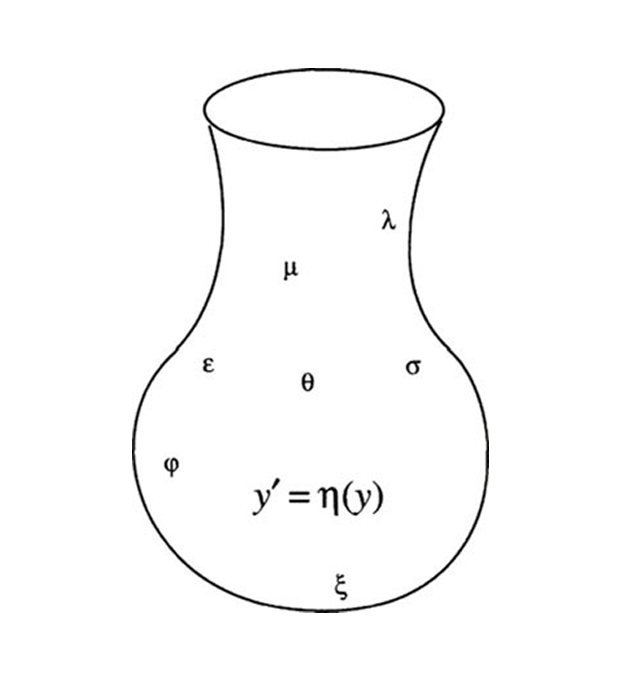
\includegraphics[width=0.5\linewidth]{Images/HW5.png}
    \end{figure}
\end{problem}
\begin{solution}
There are three jokes that we could think of. None of them funny.
    \begin{enumerate}
        \item There is no joke. Absurdist humor. Kind of like Dada art, but with humor. Pugh sounds like poo is the joke. This is like the button in season 2 of Lost that does nothing (I haven't finished the show it might do something) even though they are told the world will blow up if they don't keep pushing it.
        \item $y' =\eta(y)$ sounds like "y prime ate a y." Pugh was born in 1940, and he thinks fatshaming $y$ is real funny. This is still Biden's America Godamit.
        \item This is a reference to the poem 
        "Ode to a Grecian Urn." This is not funny for multiple reasons:
            \begin{enumerate}
                \item This is a Dad Joke. And not a good one. 
                \item Poetry.
                \item I only laugh at brainrot with Peter Griffin underneath.
            \end{enumerate}        
    \end{enumerate}
\end{solution}

\end{document}